% !TeX program = pdfLaTeX
\documentclass[12pt]{article}
\usepackage{amsmath}
\usepackage{graphicx,psfrag,epsf}
\usepackage{enumerate}
\usepackage{natbib}
\usepackage{textcomp}
\usepackage[hyphens]{url} % not crucial - just used below for the URL
\usepackage{hyperref}
\providecommand{\tightlist}{%
  \setlength{\itemsep}{0pt}\setlength{\parskip}{0pt}}

%\pdfminorversion=4
% NOTE: To produce blinded version, replace "0" with "1" below.
\newcommand{\blind}{0}

% DON'T change margins - should be 1 inch all around.
\addtolength{\oddsidemargin}{-.5in}%
\addtolength{\evensidemargin}{-.5in}%
\addtolength{\textwidth}{1in}%
\addtolength{\textheight}{1.3in}%
\addtolength{\topmargin}{-.8in}%

%% load any required packages here



% Pandoc citation processing


\begin{document}


\def\spacingset#1{\renewcommand{\baselinestretch}%
{#1}\small\normalsize} \spacingset{1}


%%%%%%%%%%%%%%%%%%%%%%%%%%%%%%%%%%%%%%%%%%%%%%%%%%%%%%%%%%%%%%%%%%%%%%%%%%%%%%

\if0\blind
{
  \title{\bf An observational study of papers published in \emph{PLOS ONE} and
studies posted to a trial registry.}

  \author{
        Nicole White \thanks{The authors gratefully acknowledge \ldots{}} \\
    School of Public Health and Social Work, QUT\\
     and \\     Thiru Balasubramaniam, Richi Nayak \\
    To add\\
     and \\     Adrian Barnett \\
    School of Public Health and Social Work, QUT\\
      }
  \maketitle
} \fi

\if1\blind
{
  \bigskip
  \bigskip
  \bigskip
  \begin{center}
    {\LARGE\bf An observational study of papers published in \emph{PLOS ONE} and
studies posted to a trial registry.}
  \end{center}
  \medskip
} \fi

\bigskip
\begin{abstract}
The text of your abstract. 200 or fewer words.
\end{abstract}

\noindent%
{\it Keywords:} 3 to 6 keywords, that do not appear in the title
\vfill

\newpage
\spacingset{1.45} % DON'T change the spacing!

\hypertarget{introduction}{%
\section{Introduction}\label{introduction}}

An ideal statistical analysis will use appropriate methods to create
insights from the data and inform the research questions. Unfortunately
many current statistical analyses are far from ideal, with many
researchers using the wrong methods, misinterpreting the results, or
failing to adequately check their assumptions \citep{2008, Leek2017}.
Some researchers take a ``mechanistic'' approach to statistics, copying
the few methods they know regardless of their appropriateness, and then
going through the motions of the analysis \citep{Stark2018}.

Many researchers lack adequate training in research methods, and
statistics is something they do with trepidation and even ignorance
\citep{Altman1994, King2019}. However, using the wrong statistical
methods can cause real harm \citep{Altman1994, Brown2018} and bad
statistical practices are being to used abet weak science
\citep{Stark2018}. Statistical mistakes are a key source of waste in
research and partly explain the current reproducibility crisis in
science \citep{Allison2016}. Even when the correct methods are used,
many researchers fail to describe them adequately, making it difficult
to reproduce the results \citep{Ernst2017, Zhou2018}. Poor statistical
methods might not be caught by reviewers, as they may not be qualified
to judge the statistics. A recent survey of editors found that only 23\%
of health and medical journals used expert statistical review for all
articles \citep{Hardwicke2020}, which was little different from a survey
from 22 years ago \citep{Goodman1998}.

There is guidance for researchers on how to write up their statistical
methods and results. The International Committee of Medical Journal
Editors recommend that researchers should: ``Describe statistical
methods with enough detail to enable a knowledgeable reader with access
to the original data to judge its appropriateness for the study and to
verify the reported results'' \citep{ICMJE2019}. More detailed guideance
is given by the SAMPL and EQUATOR guidelines
\citep{Lang2013, Altman2016} with the latter covering all apsects of the
paper. Both of these guidelines were led by Doug Altman, who spoke often
and for many years about the need for better statistical reporting. The
awareness and use of these guidelines could be improved. There were 256
Google Scholar citations to the SAMPL paper (as at 15 March 2021) which
is a good citation statistic for most papers, but is low considering the
millions of papers that use statistical analysis.

Two statisticians on this paper (AB and NW) have heard researchers admit
that they have copied-and-pasted their statistical methods sections from
other papers, regardless of whether they are appropriate. The aim of
this paper is to use text-mining methods to estimate the extent that
researchers are using cut-and-paste or `boilerplate' statistical methods
sections. Boilerplate text is that ``which can be reused in new contexts
or applications without significant changes to the original''
\citep{Wikipedia}. Use of these methods sections indicates that little
thought has gone into the statistical analysis.

\hypertarget{methods}{%
\section{Methods}\label{methods}}

\subsection{Data sources}

We used two openly available data sources to find statistical methods
sections, covering peer-reviewed journal articles and registered
clinical trial protocols.

\subsubsection{Public Library of Science (PLOS ONE)}
\label{sec:methodsPLOS}

\emph{PLOS ONE} is a large open access journal that publishes original
research across a wide range of scientific fields. Articles must be in
English. Article submissions are handled by an academic editor who
selects peer reviewers based on their self-nominated areas of expertise.
Submissions do not undergo formal statistical review. Instead, reviewers
are required to assess submissions against several publication criteria,
including whether: ``Experiments, statistics, and other analyses are
performed to a high technical standard and are described in sufficient
detail'' \citep{PLOS}. All reviewers are asked the question: ``Has the
statistical analysis been performed appropriately and rigorously?'',
with the possible responses of ``Yes'', ``No'' and ``I don't know''.

Authors are encouraged to follow published reporting guidelines such as
EQUATOR, to ensure that chosen statistical methods are appropriate for
the study design, and adequate details are provided to enable
independent replication of results.

All \emph{PLOS ONE} articles are freely accessible via the PLOS
Application Programming Interface (API). This enabled us to conduct
semi-automated searches of full-text articles and analyse data on
individual records, including text content and general attributes such
as publication date and field(s) of research. To find papers with a
statistical methods section we used targeted API searches followed by
article filtering based on section headings. The data were downloaded on
3 July 2020.

\emph{Step 1}: Targeted API searches. API searches were completed using
the R package `rplos' \citep{rplos}. Search queries targeted the
presence of analysis-related terms anywhere in the article. Search terms
combined the words ``data'' or ``statistical'' with one of:
``analysis'', ``analyses'', ``method'', ``methodology'' or
``model(l)ing''. Search terms were intended to be broad whilst keeping
search results to a manageable number for full-text review (see Step 2).
By allowing terms to appear anywhere in the article, we accounted for
the possibility of relevant text being placed in different sections, for
example, in the \emph{Material and Methods} section versus
\emph{Results}. Search results were indexed by a unique Digital Object
Identifier (DOI). Attribute data collected per DOI included journal
volume and subject classification(s).

\emph{Step 2}: Partial matching on section headings. Full text XML data
for all search results were downloaded and combined into a single
dataset, organised by DOI and subsection heading(s). Since \emph{PLOS
ONE} does not prescribe standardised headings to preface statistical
methods sections, we performed partial matching on available headings
agai

\subsubsection{Australia and New Zealand Clinical Trials Registry (ANZCTR)}
\label{sec:methodsANZCTR}

The ANZCTR was established in 2005 as part of a coordinated global
effort to improve research quality and transparency in clinical trials
reporting; observational studies can also be registered. All studies
registered on ANZCTR are publicly available and can be searched via an
online portal (\url{https://www.anzctr.org.au}).

Details required for registration follow a standardised template
\citep{ANZCTR}, which covers participant eligibility, the
intervention(s) being evaluated, study design and outcomes. The
information provided must be in English. Studies are not peer reviewed.

For the statistical methods section, researchers are asked to provide a
``brief description'' of the sample size calculations, statistical
methods and planned analyses, although this section is not compulsory
\citep{ANZCTR}. Studies are reviewed by ANZCTR staff for completeness of
key information, which does not include the completeness of the
statistical methods sections.

All studies available on ANZCTR were downloaded on 1 February 2020 in
XML format. We used all the text available in the ``Statistical
methods'' section. We also collated basic information about the study
including the study type (interventional or observational), submission
date, number of funders and target sample size. These variables were
chosen as we believed they might influence the completeness of the
statistical methods section, because we expected larger studies and
those with funding to be more complete, and we also were interested in
changes over time.

Studies prior to 2013 were excluded as the statistical methods section
appeared to be introduced in 2013. Some studies were first registered on
the alternative trial database \emph{clinicaltrials.gov} and then also
posted to ANZCTR. We excluded these studies because they almost all had
no completed statistical methods section as this section is not included
in \emph{clinicaltrials.gov}.

\subsection{Full-text processing}
\label{sec:methods-cleaning}

We applied the same text cleaning to both data sources. Text cleaning
aimed to standardise notation and statistical terminology, whilst
minimising changes to article style and formatting. \emph{R} code used
for data extraction and cleaning is available from
\url{https://github.com/agbarnett/stats_section}.

Mathematical notation including Greek letters was converted from Unicode
characters to plain text. For example, the Unicode characters
corresponding to \(\theta\) (\textless U+03B8\textgreater) were replaced
with `theta'. Similarly, common symbols outside of Unicode blocks
including `\%' (percent) and `\textless{}' (`less-than') were converted
into plain text using the `textclean' package \citep{textclean}. General
formatting was removed, this included carriage returns, punctuation
marks, in-text references (e.g.~``{[}42{]}'') centred equations, and
other non-ASCII characters. Text contained inside brackets was retained
to maximise content for analysis, with brackets removed.

We compiled an extensive list of statistical terms to standardise
descriptions of statistical methods reported across both datasets. An
initial list was compiled by calculating individual word frequencies and
identifying relevant terms that appeared at least 100 times. Further
terms were sourced from index searches of three statistics textbooks
\citep[\citet{Diggle2013},\citet{Bland2015}]{Dobson2018}. The final list
is provided as Supplementary Material. Plurals (e.g., `chi-squares')
unhyphenated (e.g., `chi square') and combined (e.g.~`chisquare') terms
were transformed to singular, hyphenated form (e.g., `chi-square').
Common statistical tests were also hyphenated (e.g., `hosmer lemeshow'
to `hosmer-lemeshow').

As a final step, common stop words including pronouns, contractions and
selected prepositions were removed. We retained selected stop words
that, if excluded, may have changed the context of statistical methods
being described, for example `between' and `against'.

nst frequently used terms in initial search results: `Statistical
analysis', `Statistical analyses', `Statistical method', `Statistics',
`Data analysis' and `Data analyses'. To determine the reliability of our
chosen filters, we manually reviewed full text data extracted for a
random sample of XXX articles that were not matched (File
S1).{[}TODO\ldots finish this thought\ldots{]}

\subsection{Clustering algorithm}

\emph{Details to come}

Results were transformed to lower case for the clustering, but examples
are given using the original capitalisation.

\subsection{Missing statistical methods sections}

The statistical methods section for the ANZCTR data was missing for some
studies and we examined if there were particular studies where this
section was more likely to be missing. We used four independent
variables of date, study type (observational or interventional), number
of funders and target sample size. We used a logistic regression model
fitted using a Bayesian paradigm. A small number of sections were
labelled as ``Not applicable'', ``Nil'' or ``None'' and we changed these
to missing.

\hypertarget{results}{%
\section{Results}\label{results}}

\hypertarget{plos-one}{%
\subsection{\texorpdfstring{\emph{PLOS ONE}}{PLOS ONE}}\label{plos-one}}

\begin{figure}
\centering
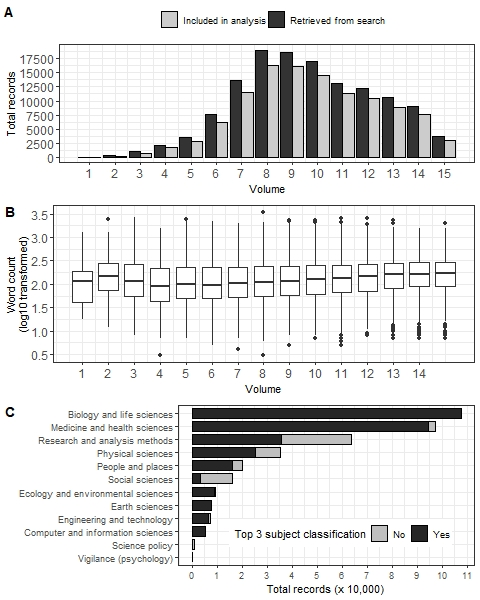
\includegraphics{figures/figure1.jpg}
\caption{\label{fig:plos-n}A: Search results by \emph{PLOS ONE} volume;
B: word count per statistical methods section included in analysis (n =
111,73); C: subject classifications assigned to full-text records
included in analysis}
\end{figure}

API searches returned 131,847 unique records, of which 111,731 (85\%)
included a statistical methods section based on our search criteria. In
the final sample, 95,518 (85\%) DOIs returned an exact match against
common section headings, including 64,133 for `statistical analysis',
13,380 for `statistical analyses' and 13,627 for `data analysis'. Among
DOIs that did not meet the partial matching criteria, initial search
terms appeared in {[}TODO{]}.

Search results varied by journal volume (Figure \ref{fig:plos-n}A). The
total number of API search results peaked at volumes 8 (n = 19,045) and
9 (n = 19,045), corresponding to years 2013 and 2014. This trend aligned
with the total number of papers published in \emph{PLOS ONE} over the
same period. The percentage of records that included a statistical
methods section by volume based on our proposed matching criteria varied
between 64\% (volume 2) and 86\% (volume 9).

The median length of statistical methods sections was 127 words (IQR: 61
to 254 words) (Figure \ref{fig:plos-n}B). 7,450 articles (7\%) had a
statistical methods section of 500 words or more. 19,461 articles (17\%)
had a statistical methods section of 50 words or less, equal to the
length of this paragraph.

All papers included Biology and life sciences (n = 107,584), Earth
sciences (n = 7,605) and/or Computer and information sciences (n =
5,190) in their top 3 subject classifications (Figure
\ref{fig:plos-n}C).

\begin{figure}
\centering
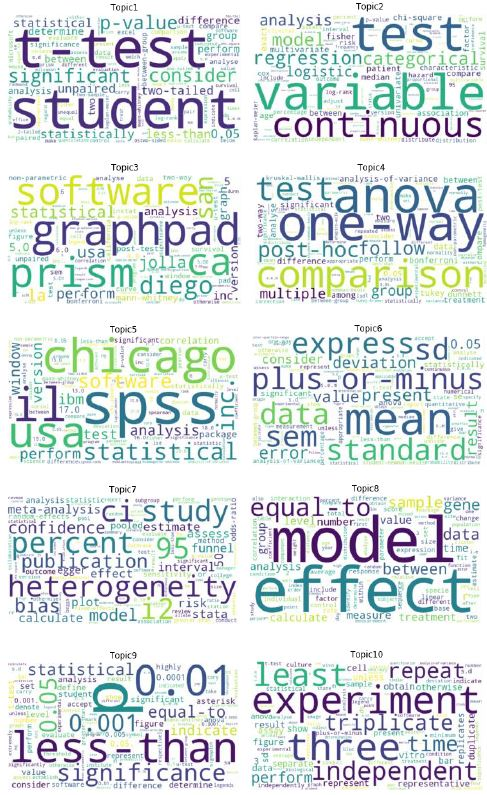
\includegraphics{figures/figure2.jpg}
\caption{\label{fig:plot-10-topics}Topic clouds summarising common terms
in \emph{PLOS ONE} statistical methods sections assuming ten clusters}
\end{figure}

We applied the clustering algorithm to the cleaned dataset, varying the
number of clusters from 1 to 50. Increasing the number of clusters
decreased cluster quality based on global goodness-of-fit measures
(Supplementary Figure 1), with average silhouette score and
within-cluster dispersion leveling off around 20 clusters. This
indicated that the data comprised one large, heterogeneous cluster and
multiple smaller clusters.

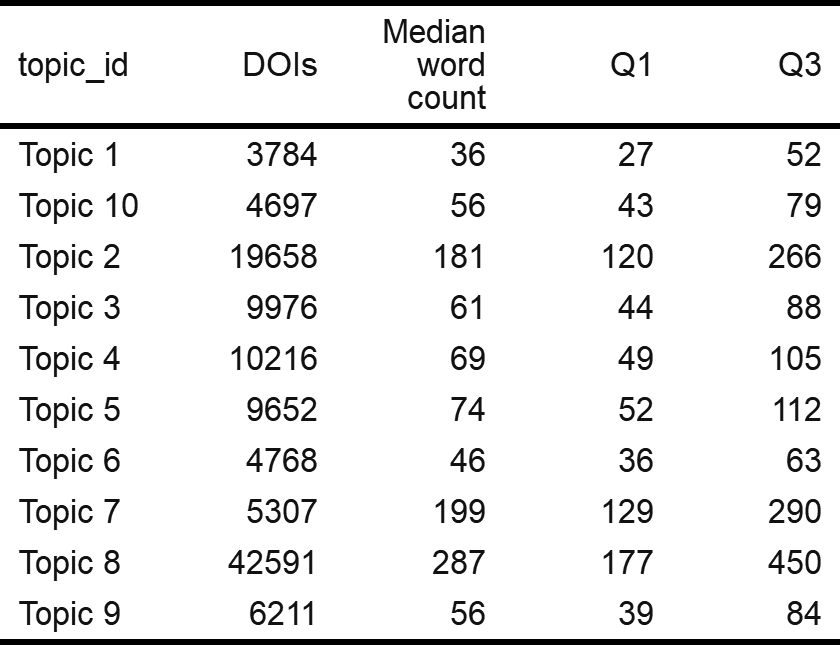
\includegraphics[width=3.75in,height=2.75in,keepaspectratio]{asa_template_files/figure-latex/unnamed-chunk-4-1.png}

The topic clouds based on ten clusters are in
Figure\textasciitilde{}\ref{fig:plot-10-topics}. Frequently occurring
words reflected the use of statistical software (Topics\textasciitilde3
and 5), descriptive statistics (Topic\textasciitilde6), group based
hypothesis testing (Topics 1 and 4) and definitions of statistical
significance (Topics\textasciitilde1 and 9). There are also statistical
methods sections associated with regression (Topic\textasciitilde2) and
meta-analysis (Topic\textasciitilde7).

Topics related to the use of statistical software differentiated between
Prism GraphPad (Topic\textasciitilde3: n = 9,879; 8.8\%) and SPSS (Topic
5: n = 9,574; 8.6\%) (Box 1). A manual review of the top matching
sections in these topics showed strong evidence of boilerplate text.
Nine out ten top matches for Topic 3 stated the use of Prism GraphPad
but did not specify which statistical methods were used; six out of ten
top matches returned the same cluster score indicating near identical
text. Top matching sections for Topic 5 included information on SPSS
version numbers and definitions of statistical significance.

\bibliographystyle{agsm}
\bibliography{references.bib}

\end{document}
